\def\mySecNum{19.4}
\mySection{\mySecNum~Monte Carlo valuation}
%-------------- start slide -------------------------------%{{{ 1 Expression in general
\begin{frame}[fragile,t]
	\begin{align*}
		V(S_0,0) = \frac{1}{n} e^{-rT}\sum_{n=1}^{n} V\left(S_T^i,T\right)
	\end{align*}
	where
	\begin{itemize}
		\item $S_T^1,\cdots, S_T^n$ are  $n$ randomly drawn time-$T$ stock prices.
		\item For European Call:
			\begin{align*}
				V(S_T^i,T) = \max\left(0,S_T^i-K\right)
			\end{align*}
		\item[] Similarly one finds the expression for European put.
	\end{itemize}
\end{frame}
%-------------- end slide -------------------------------%}}}
%-------------- start slide -------------------------------%{{{ 1 Table 19.2
\begin{frame}[fragile,t]
\begin{myexample}
	Carry out the Monte Carlo valuation of the European call under the setting of the following table:
	\begin{center}
		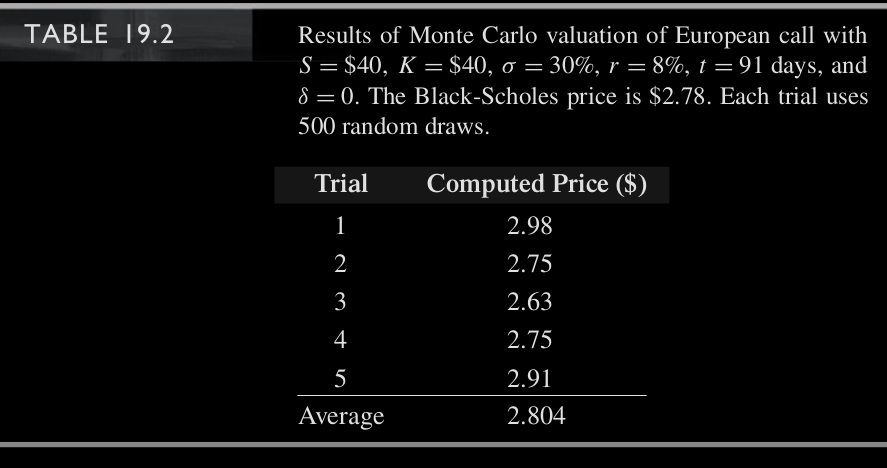
\includegraphics[scale=0.25]{figs/Table_19-2.png}
	\end{center}
\end{myexample}
\bigskip
\begin{mysol}
Check
\begin{center}
	\textcolor{gray}{codes/Table\_19-2.py}
\end{center}
\myEnd
\end{mysol}
\end{frame}
%-------------- end slide -------------------------------%}}}
%-------------- start slide -------------------------------%{{{ 1 Table 19.3
\begin{frame}[fragile,t]
\begin{myexample}
	Carry out the Monte Carlo valuation of the Asian call under the setting of the following table:
	\begin{center}
		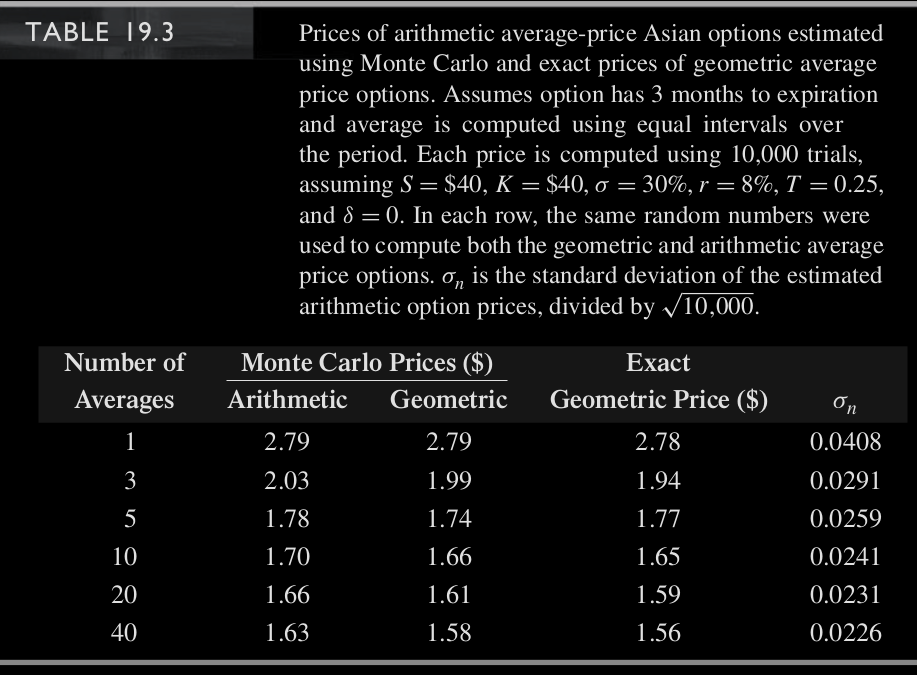
\includegraphics[scale=0.25]{figs/Table_19-3.png}
	\end{center}
\end{myexample}
\begin{mysol}
Check
\begin{center}
	\textcolor{gray}{codes/Table\_19-3.py}
\end{center}
\myEnd
\end{mysol}
\end{frame}
%-------------- end slide -------------------------------%}}}
